Για την ανάπτυξη εφαρμογών για την συσκευή Microsoft HoloLens 2, είναι απαραίτητη η εγκατάσταση συγκεκριμένων προγραμμάτων και λογισμικών από μια λίστα εργαλείων που παρέχει η Microsoft~\cite{thetuvix_2023_install,qianw211_2022_choosing}. Η επιλογή των εργαλείων γίνεται από τον προγραμματιστή ανάλογα με την εξοικείωση του με τα εργαλεία αυτά και τις γλώσσες προγραμματισμού που χρησιμοποιούν, καθώς και το διαθέσιμο υλικό (documentation). Στο παρόν κεφάλαιο, θα δοθεί μια σύντομη περιγραφή των εργαλειών που θα αξιοποιηθούν για την ανάπτυξη της εφαρμογής, καθώς και των δυνατοτήτων που παρέχουν.

\subsection{Unity}
Η Microsoft δίνει την δυνατότητα στον προγραμματιστή να επιλέξει μεταξύ τεσσάρων μηχανών (software engines) και APIs στην οποία μπορεί να υλοποιήσει την εφαρμογή του~\cite{qianw211_2022_choosing}, τα οποία παρατίθονται στον \hyperref[table:enginesAndApi]{Πίνακα~\ref*{table:enginesAndApi}}, μαζί με τη γλώσσα προγραμματισμού που χρησιμοποιεί κάθε engine ή API\@. Στα πλαίσια ανάπτυξης της εφαρμογής μας, ως μηχανή επιλέχθηκε η πλατφόρμα ανάπτυξης τρισδιάστατων εφαρμογών Unity, λόγω του πλούσιου documetation που παρέχεται από την Microsoft~\cite{qianw211_2022_unity} και από την Unity Technologies, καθώς και του υλικού και των οδηγών, που είναι διαθέσιμα στο διαδίκτυο (forums, videos κ.λ.π.) και παρεχόνται από μια ιδιαίτερα ενεργή κοινότητα.

\begin{table}[!ht]
    \caption{Διαθέσιμα engines και APIs για την ανάπτυξη εφαρμογών για το Microsoft HoloLens 2}\label{table:enginesAndApi}
    \begin{tabularx}{\textwidth}{|X|X|} %chktex-file 44
        \hline
        \textbf{Engine και API} & \textbf{Γλώσσα Προγραμματισμού} \\
        \hline
        Unity (Engine) & C\# \\
        \hline
        Unreal Engine & C++ \\
        \hline
        Custom Engine με χρήση του OpenXR API & C/C++ \\
        \hline
        Web development με χρήση του WebXR API & JavaScript \\
        \hline
    \end{tabularx}
\end{table}

Η Unity είναι μια πλατφόρμα ανάπτυξης τρισδιάστατων εφαρμογών, η οποία αναπτύχθηκε από την Over the Edge Entertainment (η οποία μετανομάστηκε σε Unity Technologies το 2007) και κυκλοφόρησε στις 8 Ιουνίου 2005. Η μηχανή, αρχικά, αναπτύχθηκε για την υλοποίηση εφαρμογών στο λειτουργικό σύστημα Mac OS X, ενώ στη συνέχεια έγινε δυνατή η ανάπτυξη σε πληθώρα πλατφορμών, όπως οι κινητές συσκευές (Android, iOS), υπολογιστές (Mac, Windows, Linux), παιχνιδοκονσόλες, πλατφόρμες εικονικής/εκτεταμένης πραγματικότητας κ.α. Η Unity επιτρέπει την ανάπτυξη τρισδιάστατων (3D), καθώς και δισδιάστατων (2D) εφαρμογών και χρησιμοποιείται σε κλάδους και βιομηχανίες, όπως η βιομηχανία βιντεοπαιχνιδιών, κινηματογράφου, ο κλάδος της αρχιτεκτονικής κ.α. Η τρέχουσα LTS έκδοση της μηχανής παιχνιδιών είναι η Unity 2023.2.1. Ωστόσο, για λόγους συμβατότητας με άλλα εργαλεία που θα χρησιμοποιηθούν, κατά την ανάπτυξη της εφαρμογής προτιμήθηκε η έκδοση Unity 2020.3.48.

Η μηχανή παιχνιδιών Unity αναπτύχθηκε σε γλώσσα προγραμματισμού C++ (runtime) και αξιοποιεί τη C\# (Unity Scripting API), μια αντικειμενοστρεφής γλώσσα προγραμματισμού, η οποία αναπτύχθηκε από τη Microsoft. Αποτελεί εφαρμογή υψηλού επιπέδου, δίνοντας στον προγραμματιστή τη δυνατότητα να υλοποιήσει μια εφαρμογή με ελάχιστη γραφή κώδικα (scripts), διαθέτοντας έτοιμες προς χρήση λειτουργίες και αντικείμενα, των οποίων η συμπεριφορά μπορεί να παραμετροποιηθεί.

Εφόσον η γλώσσα προγρμματισμού, που μπορεί να χρησιμοποιήσει ο προγραμματιστής για να αναπτύξει λειτουργίες, που δεν παρέχονται από την μηχανή, είναι η αντικειμενοστρεφής C\#, τότε βασικό στοιχείο της Unity είναι η χρήση των κλάσεων (Classes) και των αντικειμένων (Objects), με κυριότερη κλάση να είναι το \code{GameObject}~\cite{unitytechnologies_2023_gameobjects}. Όλα τα στοιχεία που μπορούμε να εντοπίσουμε σε μια εφαρμογή, όπως οι χαρακτήρες, η κάμερα, ο φωτισμός, αποτελούν αντικείμενο της κλάσης \code{GameObject}. Από μόνα τους, τα αντικείμενα αυτά δεν διαθέτουν κάποια ιδιαίτερη λειτουργία ή συμπεριφορά, αλλά λειτουργούν ως <<άδεια δοχεία>>, στα οποία προστίθενται \code{Components}~\cite{unitytechnologies_2023_introduction}. Τα \code{Components} αποτελούν τα λειτουργικά μέρη των \code{GameObjects}, καθώς είναι αυτά τα οποία καθορίζουν τη συμπεριφορά τους. Κάθε \code{GameObject} μπορεί να διαθέτει άπειρα \code{Components}, τα οποία διαθέτουν παραμέτρους, τις οποίες ο προγραμματιστής μπορεί να προσαρμόσει ανάλογα με την επιθυμητή συμπεριφορά. Ωστόσο όλα τα \code{GameObjects} διαθέτουν πάντα ένα και μόνο ένα \code{Transform} component, το οποίο καθορίζει τη θέση, περιστροφή και κλίμακα του αντικειμένου. Επιπλέον, είναι δυνατή η δημιουργία custom \code{Component} από τον προγραμματιστή με τη χρήση του Unity Scripting API, δηλαδή με τη συγγραφή αρχείων κώδικα σε C\# (C\# scripts)~\cite{unitytechnologies_2023_creating}. Ένα \code{GameObject}, επίσης, μπορεί να έχει πολλαπλά `children' \code{GameObjects}, το καθένα με τα δικά του \code{Components} και παραμετροποιήσεις. Αν ο χρήστης θέλει να χρησιμοποιήσει ένα τέτοιο σύνολο από \code{GameObjects} με τα \code{Components} που διαθέτουν, τότε, για λόγους ευκολίας, μπορεί να δημιουργήσει ένα \code{Prefab}, με βάση το οποίο δημιουργεί πολλαπλά αντίγραφα με κοινή συμπεριφορά.

\begin{figure}[!ht]
    \centering
    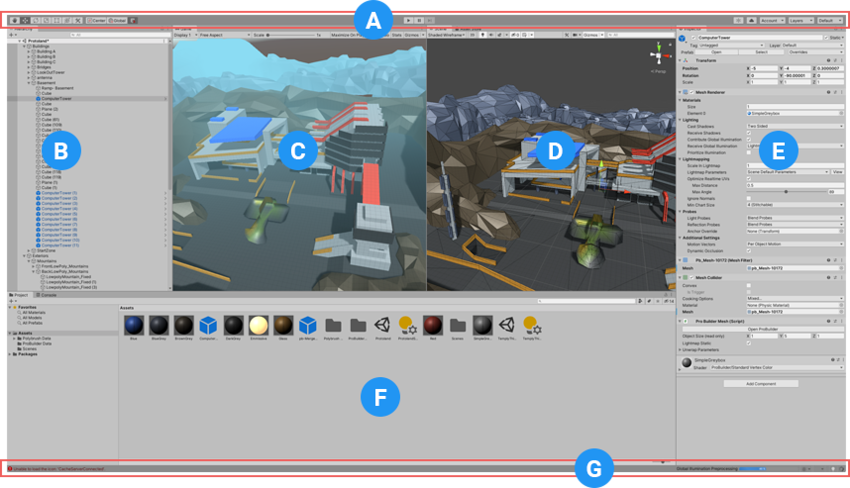
\includegraphics[width=0.9\linewidth]{images/unity_interface.png}
    \caption[Το περιβάλλον ανάπτυξης (Editor) της Unity]{Το περιβάλλον ανάπτυξης (Editor) της Unity {\footnotesize (Πηγή: docs.unity3d.com)}}\label{fig:unityInterface}
\end{figure}

Η βασική διεπαφή της Unity, όπως μπορούμε να παρατηρήσουμε και στο \hyperref[fig:unityInterface]{\schema~\ref*{fig:unityInterface}}, αποτελείται από 7 κύριες περιοχές/παράθυρα. Ειδικότερα, οι περιοχές αυτές είναι~\cite{unitytechnologies_2023_unitys}:
\begin{itemize}
    \item[(\textbf{A})] Toolbar: Το toolbar σου δίνει πρόσβαση σε ένα πλήθος εργαλείων για~\cite{unitytechnologies_2023_toolbar}: 
    \begin{itemize}
        \item τη διαχείριση των \code{GameObjects} στο Scene view
        \item τη διαχείριση της ροής στο Game view
        \item τον έλεγχο και τη διαχείριση του λογαριασμού Unity του χρήστη
        \item την επιλογή του Layer, όπου τα αντικείμενα που ανήκουν σε αυτόν θα είναι ορατά στο Scene view
        \item την επιλογή της διάταξης των παραθύρων στη διεπαφή
    \end{itemize}
    \item[(\textbf{B})] Hierarchy Window: Το παράθυρο αυτό (\hyperref[fig:unityInterfaceHierarchy]{\schema~\ref*{fig:unityInterfaceHierarchy}}) παρουσιάζει, σε μορφή λίστας, τα \code{GameObjects} που βρίσκονται σε μια σκηνή (Scene) και τη δομή αυτών. Σκηνή (Scene) αποτελεί το αρχείο που περιέχει το περιβάλλον, το μενού και τα αντικείμενα της εφαρμογής.
    
    Επιπλέον, έχουμε τη δυνατότητα να αλλάξουμε τη σειρά και το `parenting' των \code{GameObjects}, καθώς και να δημιουργήσουμε, να αντιγράψουμε ή να διαγράψουμε ένα \code{GameObject}. Τέλος, μπορούμε και να επιλέξουμε ποια \code{GameObjects} θα είναι εμφανή στο Scene view~\cite{unitytechnologies_2023_hierarchy}.
    \begin{figure}[!hb]
        \centering
        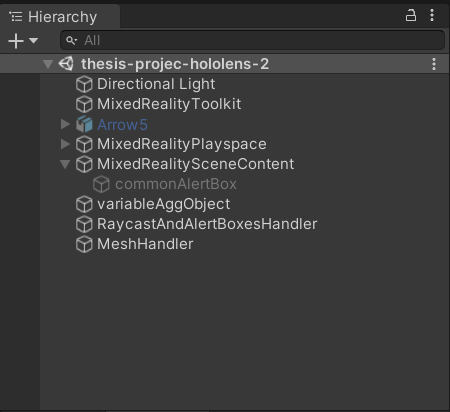
\includegraphics[width=0.5\linewidth]{images/unity_interface_hierarchy.png}
        \caption{Το Hierarchy window του Editor}\label{fig:unityInterfaceHierarchy}
    \end{figure}
    \item[(\textbf{C})] Game View: Το Game view (\hyperref[fig:unityInterfaceGameView]{\schema~\ref*{fig:unityInterfaceGameView}}) αποτελεί το παράθυρο στο οποίο παρουσιάζεται η τελική μορφή την οποία έχει η εφαρμογή μας, όπως αυτή γίνεται render από τις κάμερες (\code{Camera} component), που έχουμε στη σκηνή. Από τα κουμπιά που βρίσκονται στο toolbar μπορούμε να ορίσουμε τη ροή εκτέλεσης της εφαρμογής (έναρξη, παύση, τερματισμός κ.α.) στο Play mode. Play mode ονομάζεται η λειτουργία κατά την οποία εκτελείται η εφαρμογή και παρουσιάζεται στο Game view. Κατά την λειτουργία, μπορούν να πραγματοποιηθούν αλλαγές σε διάφορα στοιχεία, όπως \code{GameObjects}, παραμέτρους από \code{Components} κ.α., ωστόσο οι αλλαγές αυτές είναι προσωρινές και αναιρούνται, όταν ολοκληρωθεί η εκτέλεση της εφαρμογής. Τέλος, στην κορυφή του παραθύρου, υπάρχει μια εργαλειοθήκη ώστε να προσαρμόσει ο χρήστης το Game view παράθυρο και το περιεχόμενο αυτού~\cite{unitytechnologies_2023_game}.
    \begin{figure}[!ht]
        \centering
        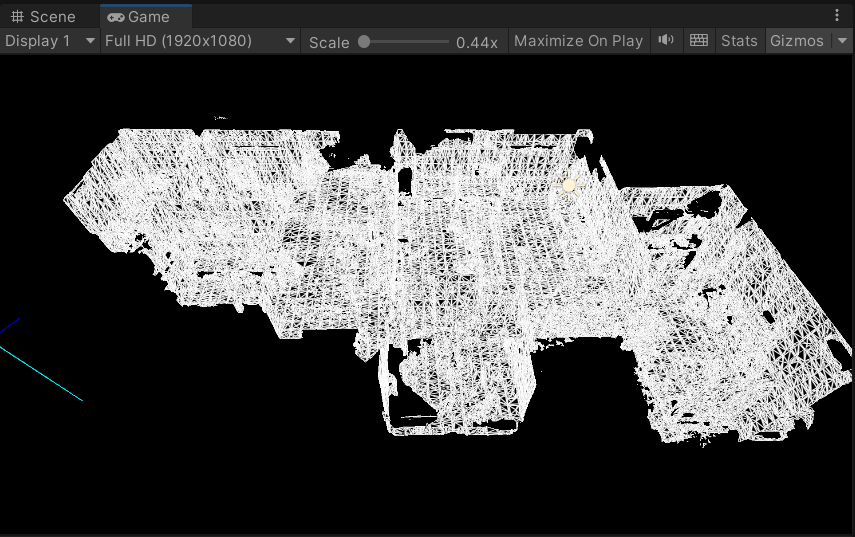
\includegraphics[width=0.9\linewidth]{images/unity_interface_game_view.png}
        \caption{Το Game view του Editor}\label{fig:unityInterfaceGameView}
    \end{figure}
    \item[(\textbf{D})] Scene View: Αποτελεί το παράθυρο (\hyperref[fig:unityInterfaceSceneView]{\schema~\ref*{fig:unityInterfaceSceneView}}), όπου ο χρήστης μπορεί να αλληλεπιδράσει με τα Game Objects τα οποία έχει εισάγει σε μια σκηνή. Στη Scene view, έχουμε μια τρισδιάστατη ή δισδιάστατη προοπτική της εφαρμογής, όπως αυτή εμφανίζεται πριν την εκτέλεση κάποιου κώδικα. Τέλος, όπως και στο Game view, στην κορυφή του παραθύρου, υπάρχει μια εργαλειοθήκη όπου ο χρήστης μπορεί να τροποποιήσει το Scene view με βάση τις ανάγκες, όπως είναι η απόκρυψη των Gizmos, η αφαίρεση του φωτισμού και η αλλαγή από 3D σε 2D προοπτική και αντίστροφα~\cite{unitytechnologies_2023_scene}.
    \begin{figure}[!ht]
        \centering
        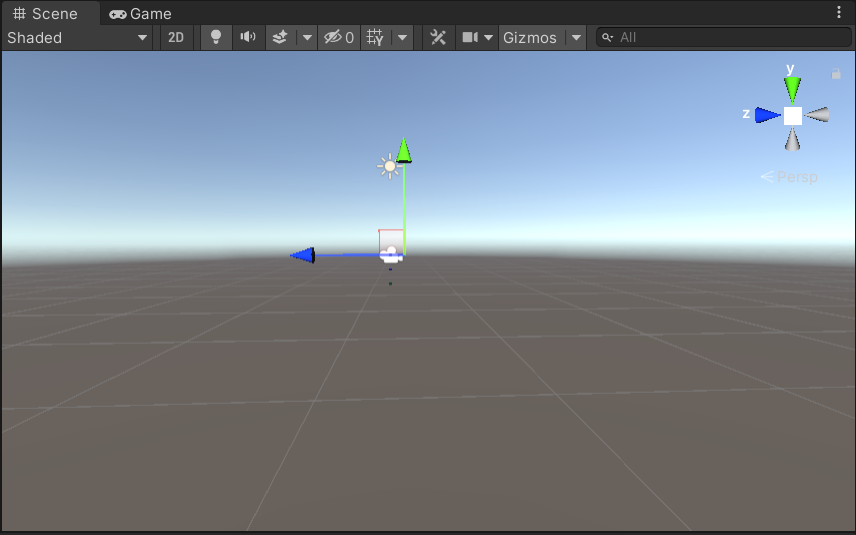
\includegraphics[width=0.9\linewidth]{images/unity_interface_scene_view.png}
        \caption{Το Scene view του Editor}\label{fig:unityInterfaceSceneView}
    \end{figure}
    \item[(\textbf{E})] Inspector Window: Απο το παράθυρο αυτό (\hyperref[fig:unityInterfaceInspector]{\schema~\ref*{fig:unityInterfaceInspector}}), ο χρήστης μπορεί να δει και να τροποποιήσει παραμέτρους πολλών στοιχείων του Editor, όπως είναι τα \code{GameObjects}, τα \code{Componetns}, τα υλικά (Materials), τα Assets, καθώς και ρυθμίσεις του Editor. Επιλέγοντας κάποιο από τα ανωτέρω στοιχεία, στον Inspector, εμφανίζονται όλοι οι παράμετροι, σχετικές με το το στοιχείο αυτό, τις οποίες μπορεί να αλλάξει ο χρήστης. Για παράδειγμα, αν επιλεχθεί ένα \code{GameObject}, τότε εμφανίζονται όλα τα \code{Components} που έχουν προστεθεί σε αυτόν. Αν κάποιο από τα \code{Components} αποτελεί Script που έχει δημιουργήσει ο χρήστης, τότε στον Inspector παρουσιάζονται οι public μεταβλητές του αρχείου αυτού~\cite{unitytechnologies_2023_inspector}.
    \begin{figure}[!ht]
        \centering
        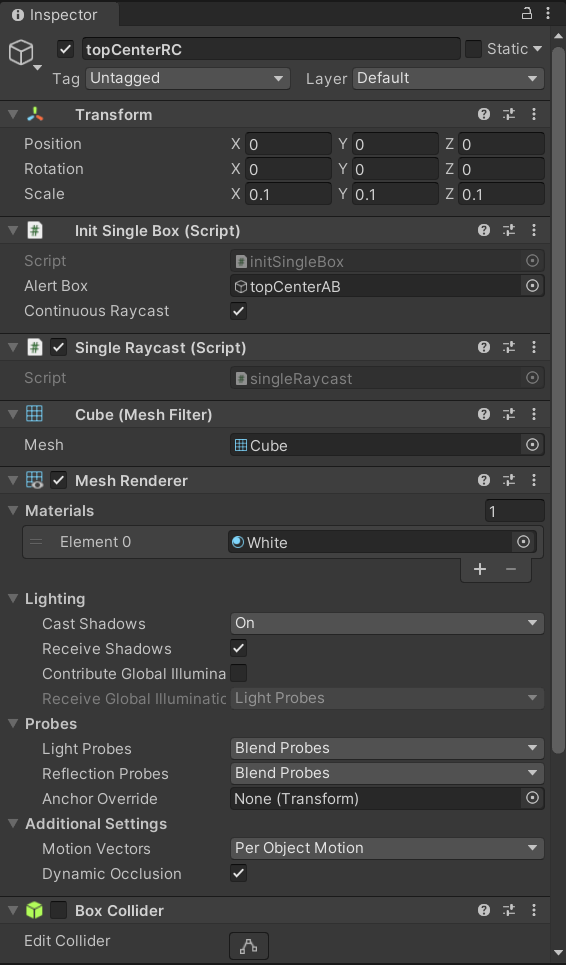
\includegraphics[width=0.5\linewidth]{images/unity_interface_inspector.png}
        \caption{Το Inspector window του Editor}\label{fig:unityInterfaceInspector}
    \end{figure}
    \item[(\textbf{F})] Project Window: Στο συγκεκριμένο παράθυρο εντοπίζονται όλα τα αρχεία, τα οποία σχετίζονται με την εφαρμογή, που υλοποιεί ο χρήστης. Ο χρήστης μπορεί να ανατρέξει στο παράθυρο αυτό σε περίπτωση που αναζητεί κάποιο Asset, το οποίο έχει ξαναχρησιμοποιήσει ή έχει αποθηκεύσει σε κάποιο φάκελο του project~\cite{unitytechnologies_2023_project}.
    
    Το Asset είναι οποιοδήποτε αντικείμενο χρησιμοποιείται κατά την ανάπτυξη της εφαρμογής, όπως είναι ένα αρχείο ήχου, μια εικόνα, ένα 3D μοντέλο~\cite{unitytechnologies_2023_asset}. Αυτά τα assets μπορούν να έχουν δημιουργηθεί από το χρήστη ή από ένα τρίτο άτομο και έχουν αποκτήθει από το χρήστη από καταστήματα, όπως το Unity Asset Store.

    Τέλος, όπως και σε άλλες περιοχές του Editor, στην κορυφή του παραθύρου υπάρχει μια εργαλειοθήκη, που επιτρέπει στο χρήστη να προσθέσει Assets στον τρέχοντα φάκελο ή να αναζητήσει κάποιο Asset με χρήση διάφορων φίλτρων~\cite{unitytechnologies_2023_project}.
    \begin{figure}[!hb]
        \centering
        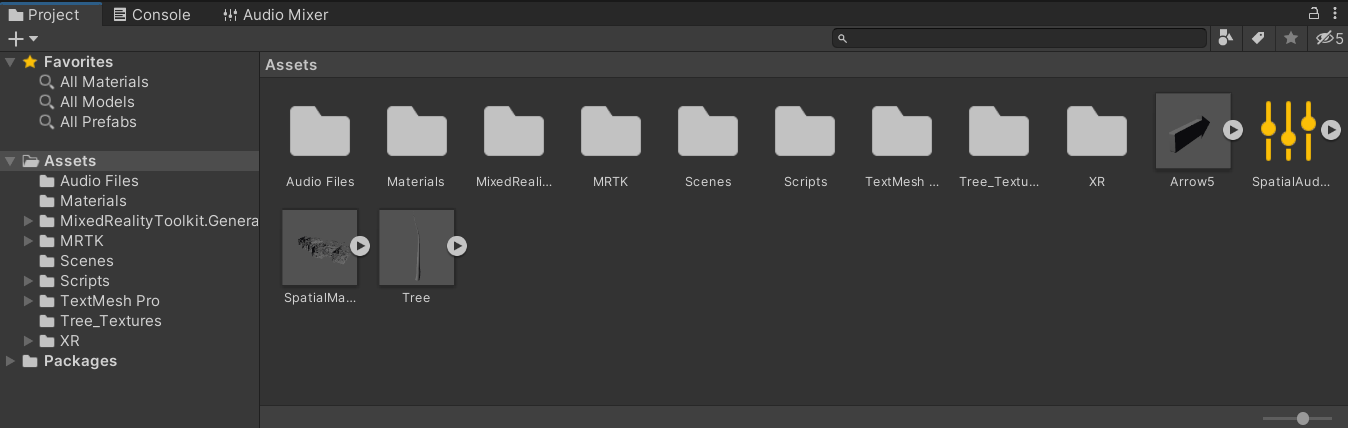
\includegraphics[width=1\linewidth]{images/unity_interface_project.png}
        \caption{Το Project window του Editor}\label{fig:unityInterfaceProject}
    \end{figure}
    \item[(\textbf{G})] Status Bar: Στο κάτω μέρος του Editor εντοπίζεται η μπάρα κατάστασης (Status Bar) (\hyperref[fig:unityInterfaceStatusBar]{\schema~\ref*{fig:unityInterfaceStatusBar}}), η οποία ενημερώνει σχετικά με την κατάσταση του Editor ή διαφόρων εργασιών που επιτελεί. Ειδικότερα, παρουσιάζεται μια προεπισκόπηση του τελευταίου μηνύματος, προειδοποίησης ή σφάλματος που καταγράφηκε στην κονσόλα (Console). Επίσης, αν επιτελείται κάποια εργασία, εμφανίζεται μια μπάρα προόδου της εργασίας αυτής. Τέλος, στο δεξί μέρος του status bar, υπάρχουν ορισμένα κουμπιά και ενδείξεις, που επιτρέπουν στο χρήστη~\cite{unitytechnologies_2023_status}:
    \begin{itemize}
        \item να αλλάξει ανάμεσα σε λειτουργία Debug και Release, το οποίο επηρεάζει την βελτιστοποίηση του κώδικα
        \item να ελέγξει την κατάσταση του cache server
        \item να ελέγξει την κατάστηση του Global illumination
        \item να ελέγξει την τρέχουσα κατάσταση του Editor, σε περίπτωση που αυτός πραγματοποιεί compilation αρχείων C\# ή άλλες ασύγχρονες εργασίες
    \end{itemize}
    \begin{figure}[!hb]
        \centering
        
\includegraphics[width=1\linewidth]{images/unity_interface_status_bar.png}
        \caption{Το Status bar του Editor}\label{fig:unityInterfaceStatusBar}
    \end{figure}
\end{itemize}

\subsection{Microsoft Visual Studio}
Το Microsoft Visual Studio αποτελεί το κύριο ολοκληρωμένο περιβάλλον ανάπτυξης (Integrated Development Environment, IDE) για την ανάπτυξη εφαρμογών στη Unity, όπως είναι οι εφαρμογές για τη συσκευή HoloLens~\cite{thetuvix_2023_install}. Κατά τη δημιουργία ενός project στη Unity, δημιουργείται ένα Visual Studio Project. Ο συγκεκριμένος editor μπορεί να χρησιμοποιηθεί για τη συγγραφή κώδικα σε γλώσσα C\#, για το compilation των αρχείων κώδικα και το build του project, αλλά και για την αποσφαλμάτωση (debugging) του κώδικα. Τέλος, μέσω του Visual Studio, είναι δυνατό η φόρτωση του project στη συσκευή~\cite{vtieto_2022_using}. Ωστόσο, αυτή είναι μια ιδιαιτέρως χρονοβόρα διαδικασία, η οποία δημιουργεί επιπλέον καθυστερήσεις στη ανάπτυξη της εφαρμογής, όπου οι συχνές αλλαγές του κώδικα και οι δοκιμές αποτελούν συχνό φαινόμενο. Για το λόγο αυτό, η μεταφόρτωση της εφαρμογής πραγματοποιείται μέσω του εργαλείου Holographic Remoting που προσφέρει το MRTK (\hyperref[subsec:mrtk]{Κεφάλαιο~\ref*{subsec:mrtk}}) μέσω της Unity.

Στα πλαίσια της παρούσας διπλωματικής εργασίας, εγκαταστάθηκε η έκδοση του προγράμματος Visual Studio 2019, καθώς και τα απαιραίτητα workloads για την ανάπτυξη εφαρμογών μικτής πραγματικότητας στη Unity.

\subsection{Mixed Reality Toolkit}\label{subsec:mrtk}
Το Mixed Reality Toolkit (MRTK) αποτελεί μια εργαλειοθήκη, η οποία αναπτύχθηκε από την Microsoft, ενσωματώνεται σε project στη Unity ως package και έχει ως σκόπο να διευκολύνει τον προγραμματιστή στην ανάπτυξη εφαρμογών μικτής πραγματικότητας, παρέχοντας μια σειρά από εργαλεία. Πιο συγκεκριμένα, παρέχει σημαντικά \code{GameObjects} και \code{Components}, τα οποία μπορούν να χρησιμοποιηθούν σε ένα εικονικό περιβάλλον ή σε αντικείμενα που υπάρχουν σε αυτόν.

Επίσης, δίνει τη δυνατότητα στο χρήστη να πραγματοποιήσει μια προσομοίωση της χρήσης της εφαρμογής μέσω του editor της Unity, χωρίς τη φόρτωση του project σε συσκευή HoloLens. Ωστόσο, στην περίπτωση αυτή, δεν είναι πάντα λειτουργικά όλα τα στοιχεία μικτής πραγματικότητας που έχουμε προσθέσει στο project και προσφέρει το MRTK~\cite{polarkev_2022_mrtk2unity}.

Όπως αναφέρθηκε, το MRTK προστίθεται ως package σε ένα Unity project. Αυτό με τη χρήση του εργαλείου Mixed Reality Feature Tool, το οποίο αναπτύχθηκε επίσης από τη Microsoft. Μέσω του εργαλείου αυτού, μπορεί ο χρήστης να αναζητήσει και να προσθέσει στο Unity project του εργαλεία και components χρήσιμα για εφαρμογές μικτής πραγματικότητας~\cite{seankerawala_2022_welcome}.

Για την ανάπτυξη της εφαρμογής μας εγκαταστήσαμε, μέσω του Mixed Reality Feature Tool, το MRTK 2.7.3, καθώς και τα packages Mixed Reality OpenXR plugin και Microsoft Spatializer.

% \subsection{HoloLens Emulator}
% Σε περίπτωση που δεν είναι εφικτή η χρήση μιας φυσικής συσκευής HoloLens, τότε είναι δυνατή η δοκιμή μιας εφαρμογής εικονικής πραγματικότητας με τη χρήση του προγράμματος HoloLens Emulator, το οποίο ανέπτυξε η Microsoft. 